\chapter{Introduzione}

    La comunicazione fra individui avviene in svariati modi, ad esempio attraverso il linguaggio verbale ed il linguaggio visivo (o linguaggio visuale).
    \newline
    Un linguaggio visuale non è altro che una forma di comunicazione, detta comunicazione visuale, che fa uso di simboli grafici o immagini. Simboli grafici, immagini e mappe sono esempi di elementi utilizzati all'interno della comunicazione visiva (o comunicazione visuale) che necessitano di un contesto per essere descritte in modo naturale. Spesso quest'ultima risulta essere molto più immediata e di facile comprensione rispetto alla tradizionale comunicazione verbale composta di lettere e parole.
    \newline
    In questa tesi presento \textbf{TiveJS}, un'estensione della piattaforma \href{https://www.draw.io/}{draw.io}, che sfrutta  simboli e  definizioni semantiche per il riconoscimento dei linguaggi diagrammatici e la traduzione di questi in altri linguaggi.

    \section{Motivazioni}
        La piattaforma già esistente, LoCoMoTiVE che implementa il freamework Local Context, si basa su un meccanismo client-server.
        \newline
        Il client è formato dalla piattaforma draw.io, opportunamente modificata, per la creazione di sentenze visuali.
        Il server è stato implementato in Java utilizzando i servlet per il riconoscimento e la traduzione delle sentenze visuali.
        Il funzionamento è molto semplice: il client esegue una chiamata HTTP di tipo POST contenute al suo interno un grafo o un diagramma, creato attraverso l'utilizzo di simboli ad hoc, in formato XML.~Una volta ricevuta la sentenza visuale, essa è interpretata dal server che applica le definizioni per poi restituire la traduzione semantica oppure dei messaggi di errore.
        \newline
        Le motivazioni che hanno portato alla creazione di un nuovo tool sono varie: rendere l'applicazione più scalabile e più veloce limitando l'interazione con il server a semplici accessi a pagine statiche; l'aggiornamento di TiVe all'ultima versione di draw.io; essendo il core di TiveJS scritto completamente in JavaScript, ora si integra perfettamente con la piattaforma estesa e con la manipolazione del grafo.
        Le definizioni dei linguaggi ora sono in formato JSON rendendo ancora più alta l'interoperabilità dei sistemi. 

        \section{Linguaggi visuali}

            In questa sezione entrerò nel dettaglio dei Linguaggi Visuali, andando ad illustrare quali sono le principali differenze tra un linguaggio visuale ed uno verbale, i componenti che lo compongono e in quali casi o contesti un linguaggi visivo è più efficace rispetto ad uno verbale.

            \subsection{Linguaggio verbale}
                Il linguaggio verbale è un gruppo di elementi, come suoni e parole, che messi insieme formano frasi e infine permettono la comunicazione fra individui. Da questo deriva la comunicazione verbale che è quindi costituita dalle parole usate quando parliamo o scriviamo.

            \subsection{Componenti}
                Ogni linguaggio è formato da un proprio insieme di componenti. Un linguaggio visuale si distingue principalmente dal linguaggio verbale per i componenti da cui è formato. Il linguaggio visivo si basa su simboli grafici o immagini, elementi che il cervello umano interpreta e trasforma in concetti, linguaggio verbale ed emozioni. Quindi se il linguaggio visuale è costituito da testo e parole per la formazioni di frasi, il linguaggio visivo è formato da simboli e disegni per formare sentenze visive.
                Una componente fondamentale di un linguaggio visuale è il contesto che viene dato ad ogni simbolo appartenente ad una frase visiva.
                \begin{figure}[htbp]
                    \centering
                    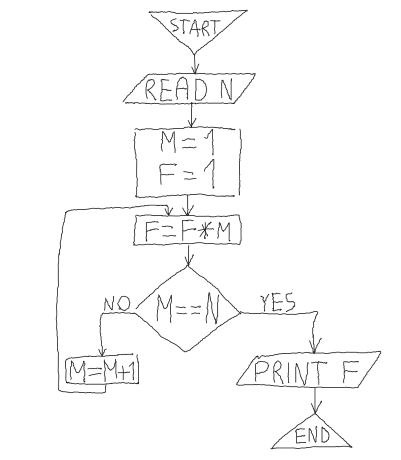
\includegraphics[scale=0.6]{Figure/diagram.PNG}
                    \caption{Esempio di sentenza visiva, da~\cite{localcontext_recognition}}
                    \label{fig:diagram}
                \end{figure}
                Ad esempio, come possiamo notare avvalendoci del disegno in figura~\ref{fig:diagram}, senza un contesto le forme grafiche sono soltanto simboli connessi fra loro da delle frecce. Invece, dando una definizione ai simboli può essere interpretato come un diagramma di flusso o \textit{Flowchart}\footnote{Il diagramma di flusso (o \textit{Flowchart}), in informatica, è una rappresentazione grafica delle operazioni da eseguire per l'esecuzione di un algoritmo.}.

            \subsection{Vantaggi}
                I vantaggi possono essere molteplici, innanzitutto un linguaggio visuale può essere molto più efficace e di facile comprensione rispetto al linguaggio verbale per via della sua semplicità e naturalità. Non ha lingue o convenzioni in quanto un disegno o un'immagine non dipende da lingue o standard.

    \section{Organizzazione della Tesi}
        Nel capitolo 2 illustrerò i lavori correlati al mio progetto di tesi.
        Nel capitolo 3 parlerò del Local Context e delle corrispondenti specifiche sintattiche e semantiche. 
        Nel capitolo 4 introdurrò il risultato del mio lavoro di tesi, TiveJS e le sue funzioni, e illustrerò  i dettagli dell'implementazione e le tecnologie usate. 
        Nel capitolo 5 illustrerò un esempio d'utilizzo. 
        Nel capitolo 6 presenterò possibili sviluppi futuri dell'applicazione e le conclusioni.